\documentclass[12pt]{report}
\usepackage[left=2.5cm,right=2.5cm,top=3cm,bottom=3cm]{geometry}
\usepackage{fancyhdr}
\usepackage{etoolbox}
\usepackage{titlesec}
\usepackage{titling} % Para personalizar el título
\usepackage{graphicx}
\usepackage{hyperref}
\usepackage{amsmath}
\usepackage{amssymb}
\usepackage{circuitikz} % Para dibujar circuitos
\usepackage{indentfirst}
\usepackage{relsize}

\geometry{a4paper}

% Configuración de cabecera y pie de página
\pagestyle{fancy}
\fancyhf{} 
\fancyhead[L]{UTN-FRC}
\fancyhead[C]{FÍSICA 2: TPL3}
\fancyhead[R]{2R3}
\renewcommand{\headrulewidth}{0.4pt}
\fancyfoot[C]{\vfill\thepage}

% Cambio en el estilo de las páginas de capítulo
\patchcmd{\chapter}{\thispagestyle{plain}}{\thispagestyle{fancy}}{}{}

% Tamaños de fuente para matemáticas
\DeclareMathSizes{12}{13}{8}{8}
\newcommand {\LEpsilon}{\mathlarger{\mathlarger{\varepsilon}}}

% Configuración del título del documento
\title{%
  \fontsize{25}{30}\selectfont Universidad Tecnológica Nacional \\
  \fontsize{22}{30}\selectfont Física 2 \\
  \fontsize{18}{25}\selectfont TPL3: Resistividad
}
\author{
  Franco Palombo - 401910\\
  Gaston Grasso - 401892\\
  Ignacio Gil - 401891\\
  Santino Noccetti - 405947\\
  Agustin Suppo - 400296\\
  Pablo Gabriel Moyano - 403337\\
}
\date{19 / 06 / 2024}

% Formato de títulos y secciones
\titleformat{\chapter}[block]
  {\normalfont\huge\bfseries}{}{0pt}{\Huge}
\titlespacing*{\chapter}{0pt}{-30pt}{20pt}

\titleformat{\section}[block]
  {\normalfont\Large\bfseries}{}{0pt}{\Large}
\titlespacing*{\section}{0pt}{3.5ex plus 1ex minus .2ex}{2.3ex plus .2ex}

\titleformat{\subsection}[block]
  {\normalfont\large\bfseries}{}{0pt}{\large}
\titlespacing*{\subsection}{0pt}{3.25ex plus 1ex minus .2ex}{1.5ex plus .2ex}

\begin{document}
\maketitle
\chapter{Ejercicio 1}
\vspace{-0.2cm}
Se confeccionó el siguiente circuito en laboratorio:
\noindent
\begin{figure}[h]
  \centering
  \begin{minipage}{0.65\textwidth}
    \centering
    \begin{circuitikz}
      % Dibujar la fuente de voltaje
      \draw (0,0) to[battery1, l=\Large$\LEpsilon$, invert] (0,3)
      % Dibujar las resistencias en serie
      to[R, l=$R_1$] (3,3)
      to[R, l=$R_2$] (6,3)
      to[R, l=$R_3$] (9,3)
      % Conectar la última resistencia a tierra y cerrar el circuito
      -- (9,0) -- (0,0);
    \end{circuitikz}
  \end{minipage}\hfill
  \begin{minipage}{0.35\textwidth}
    \centering
    (Valores teoricos)
    $$\LEpsilon = 16V$$
    $$R_1 = 50\Omega$$
    $$R_2 = 35\Omega$$
    $$R_3 = 70\Omega$$
  \end{minipage}
\end{figure}

\section{Mediciones}
Con la fuente desconectada, se midieron los valores de las distintas resistencias individualmente,
y luego la resistencia equivalente del circuito. Obteniendo los siguientes valores:

$$R_1 = 48,\!5\Omega \hspace{5mm} R_2 = 34,\!1\Omega \hspace{5mm} R_3 = 69\Omega$$

\noindent
\begin{figure}[h]
  \centering
  \begin{minipage}[h]{0.3\textwidth}
    \centering
    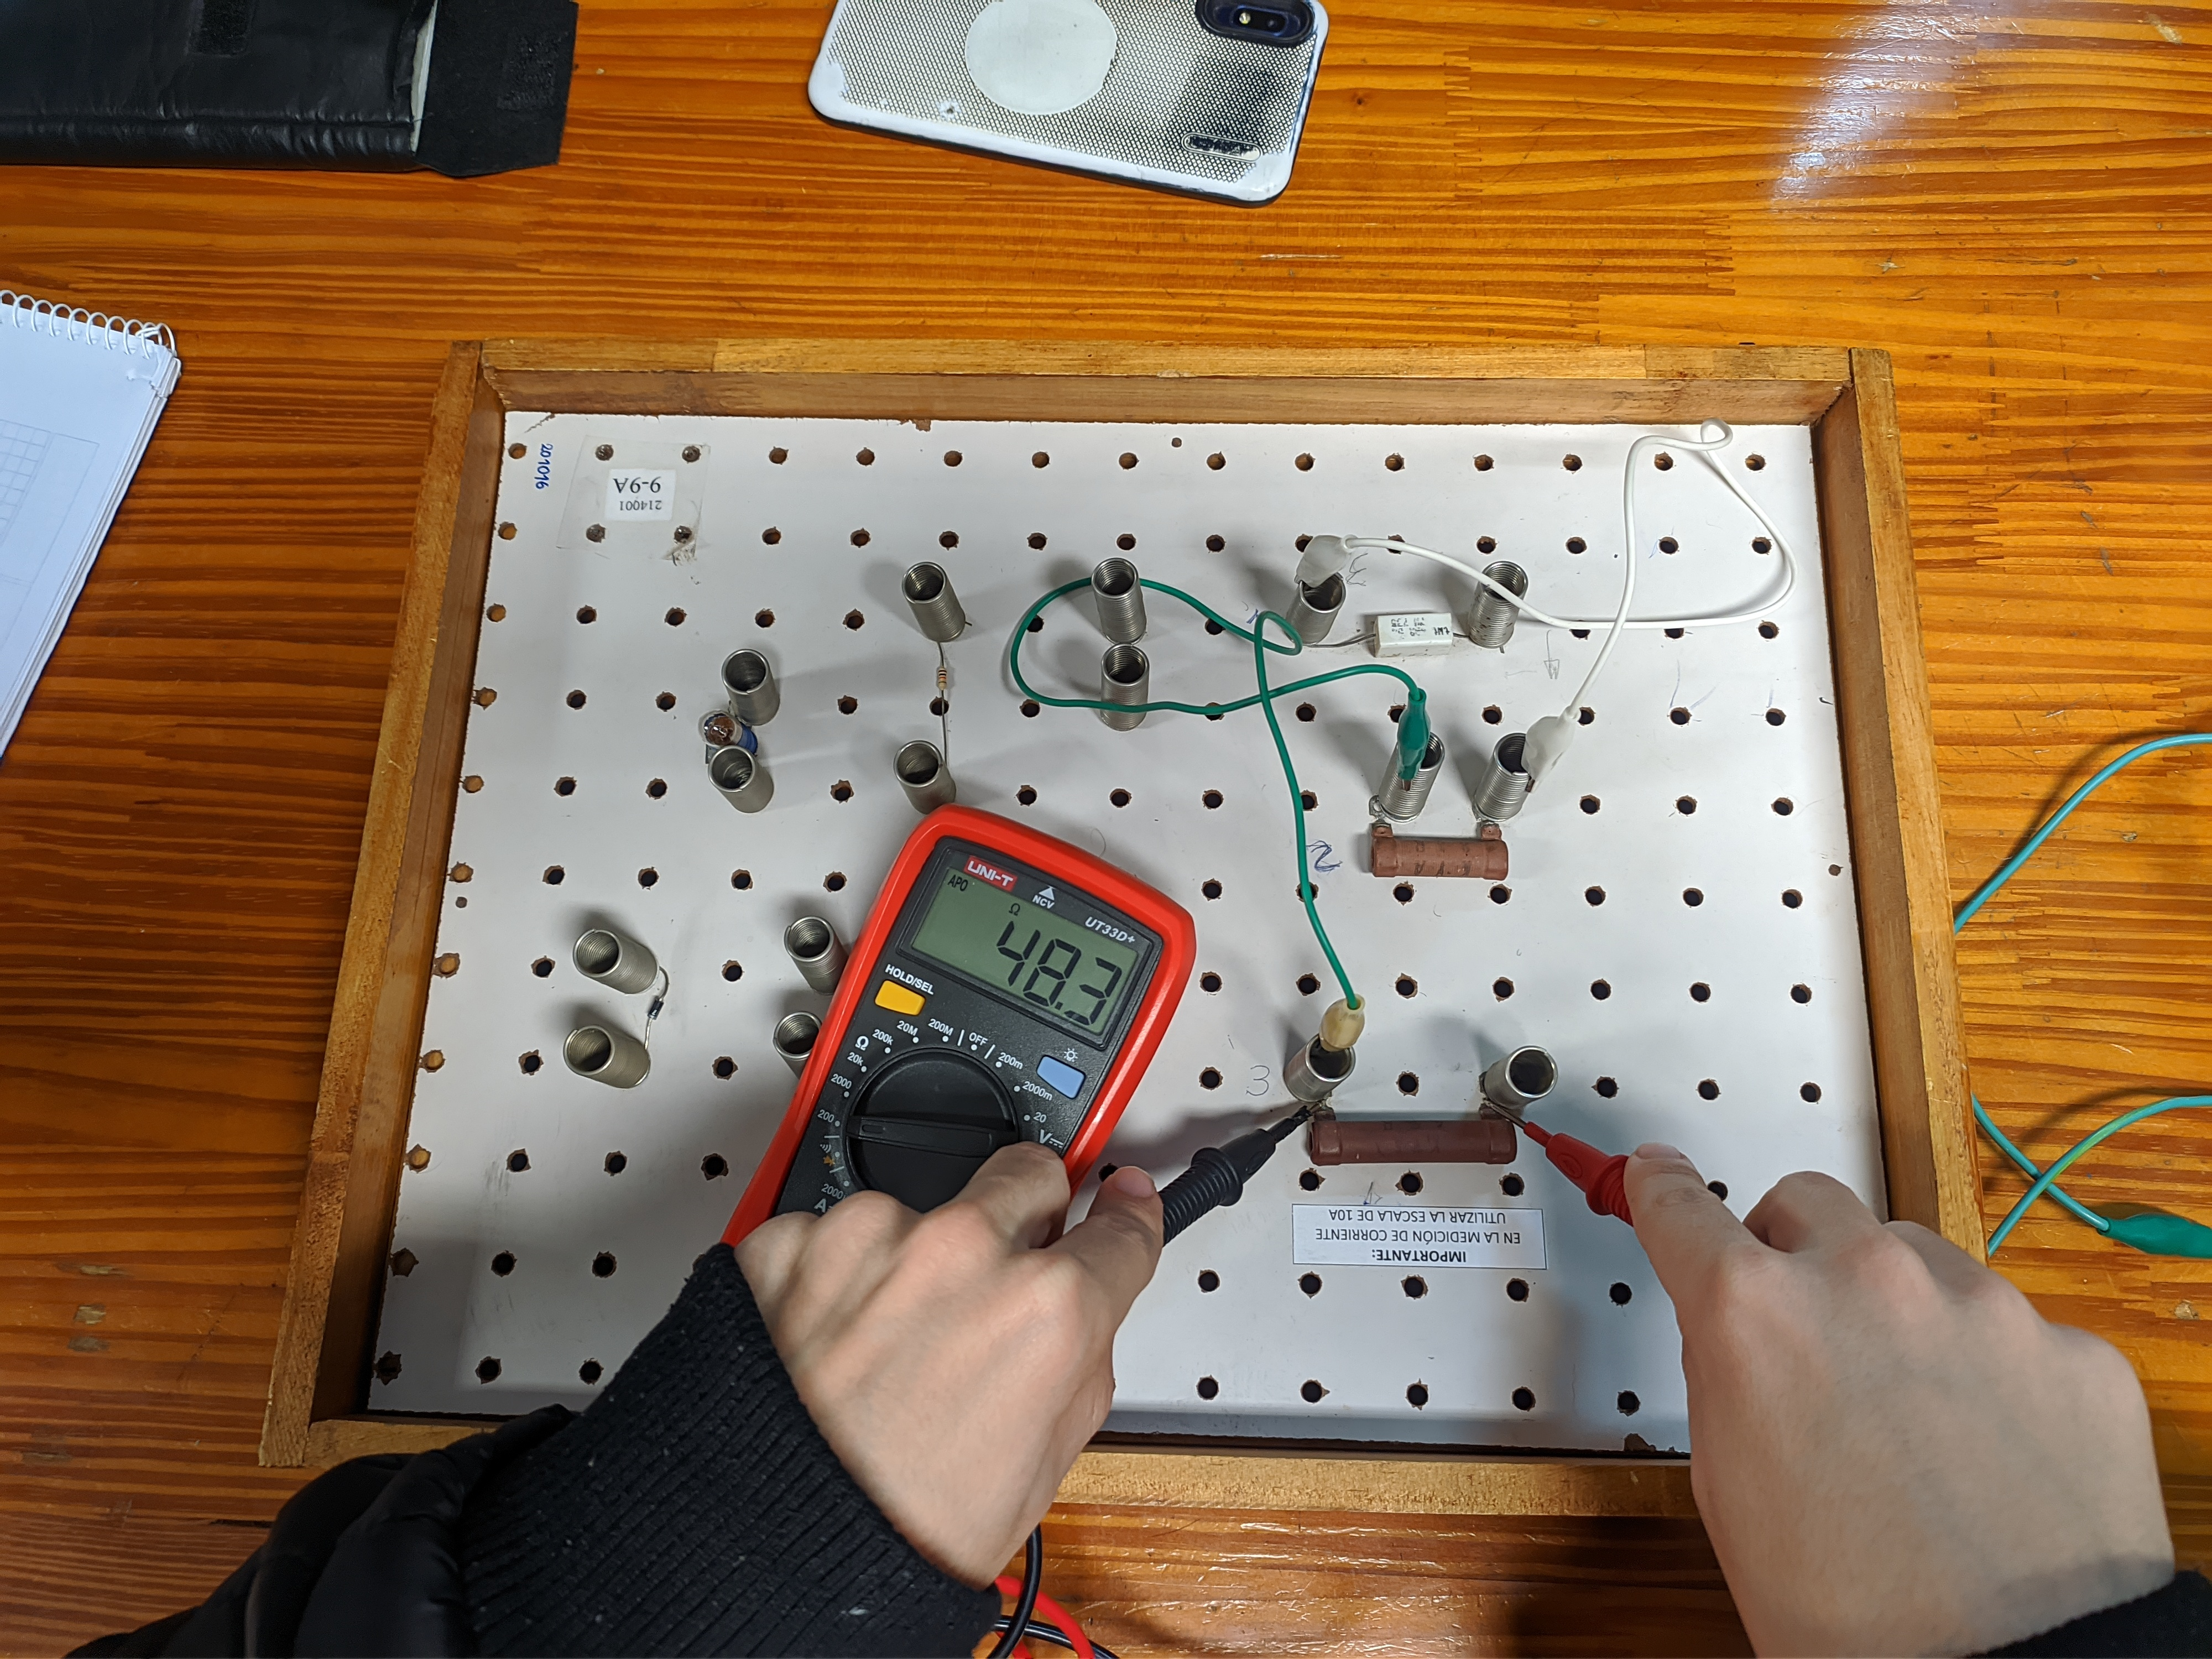
\includegraphics[width=1\textwidth]{./pictures/SERIE_R1.jpg}
    \textit{Medicion $R_1$.}
  \end{minipage}\hskip 5mm
  \begin{minipage}[h]{0.3\textwidth}
    \centering
    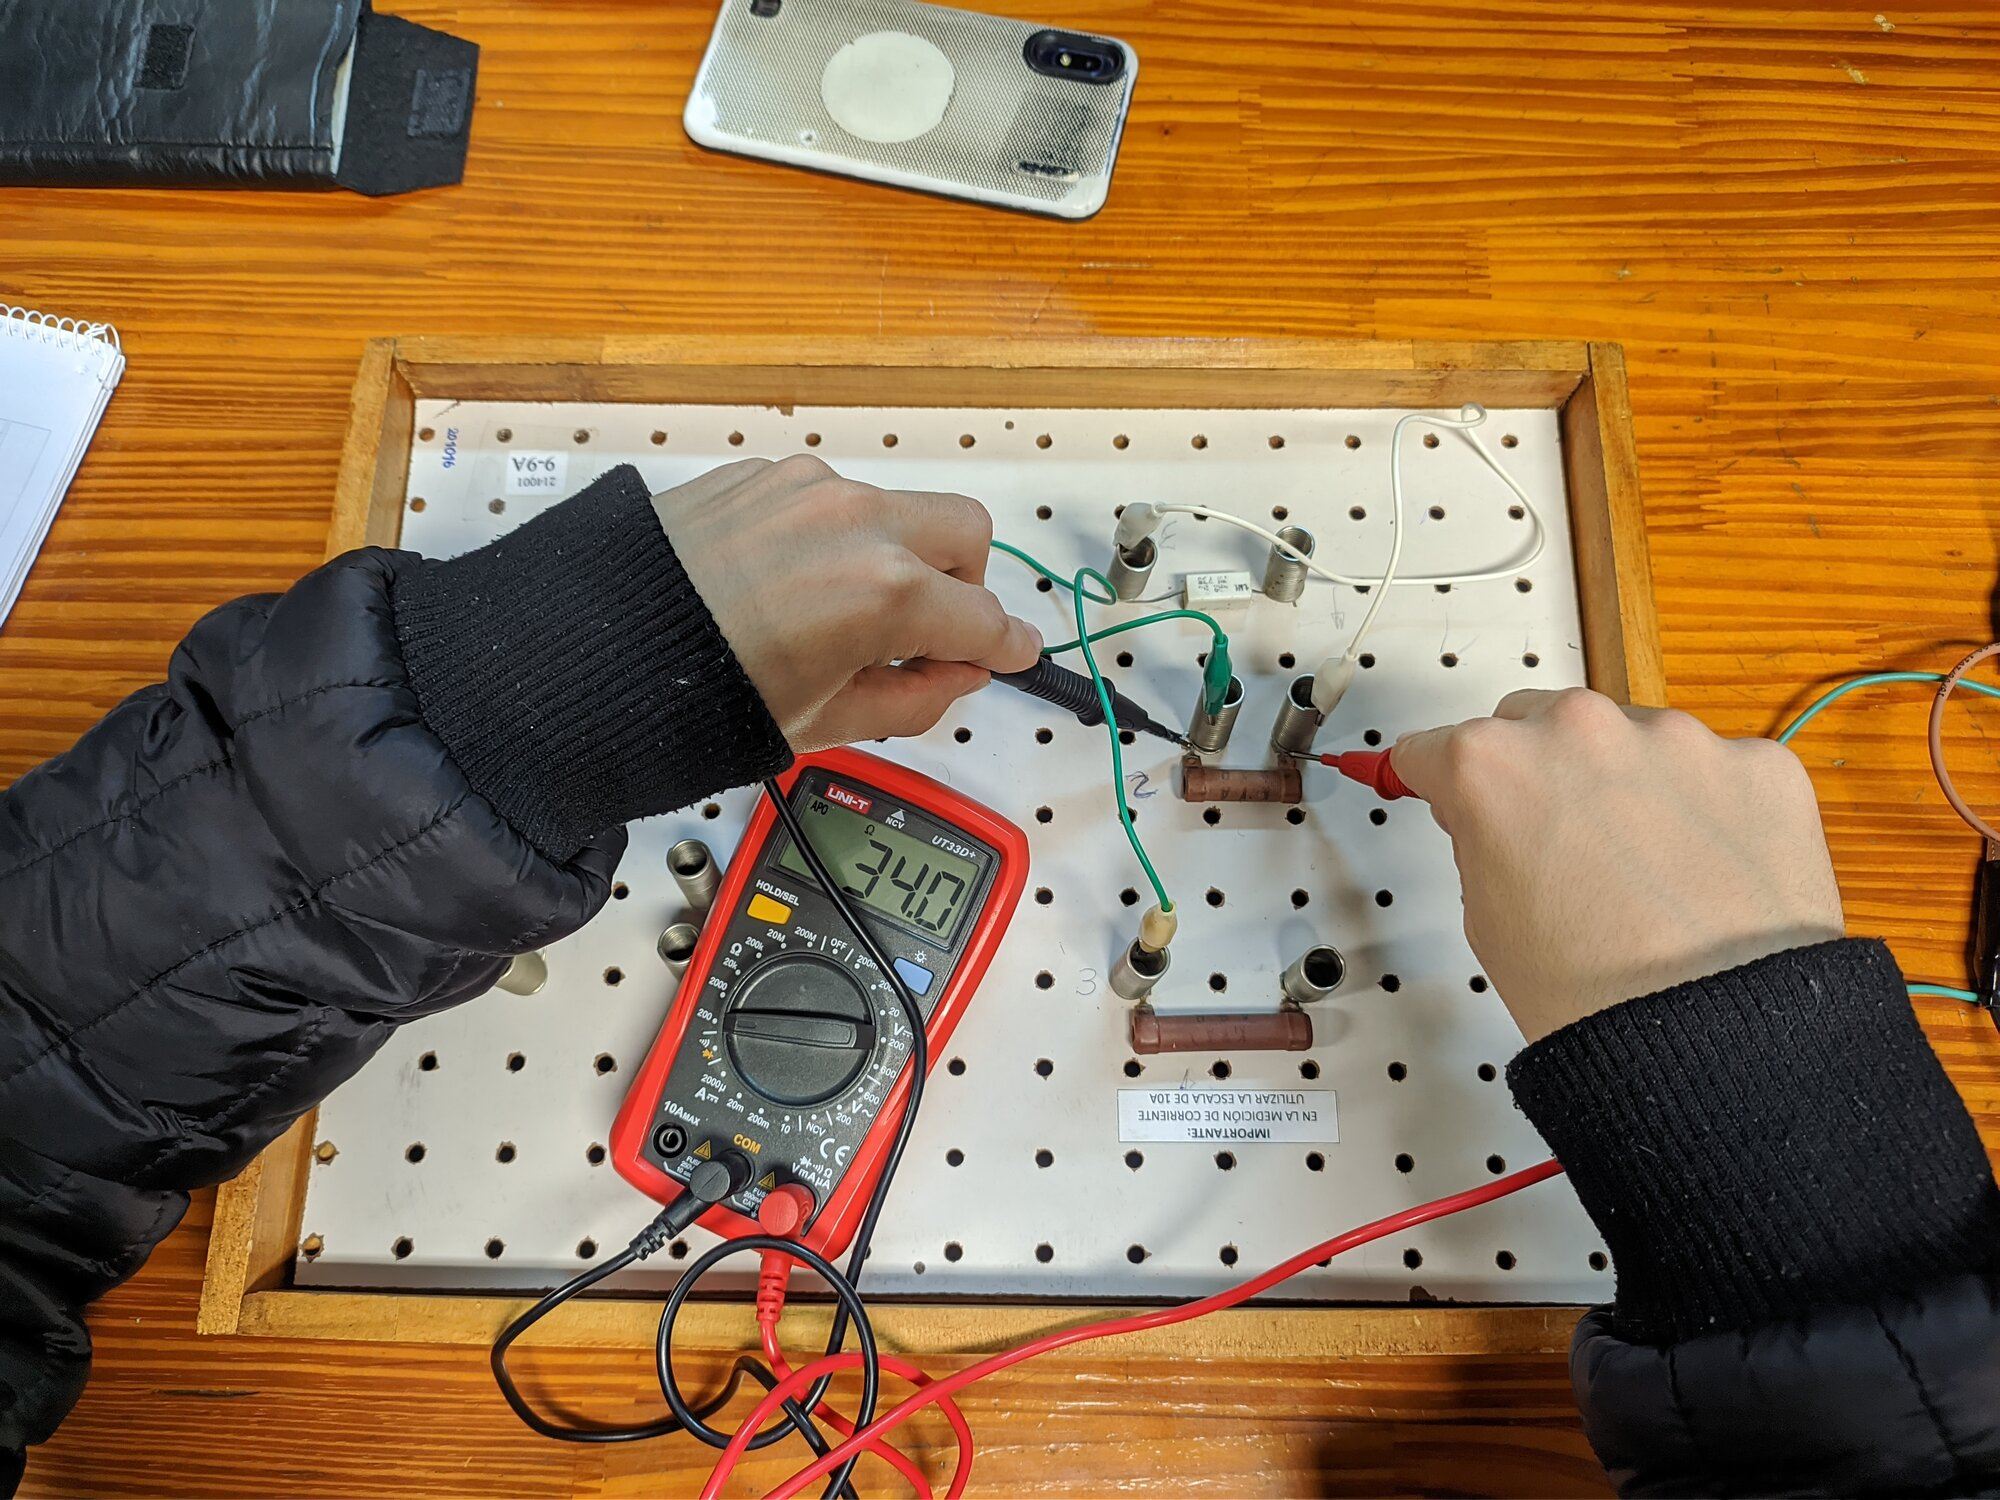
\includegraphics[width=1\textwidth]{./pictures/SERIE_R2.jpg}
    \textit{Medicion $R_2$.}
  \end{minipage}\hskip 5mm
  \begin{minipage}[h]{0.3\textwidth}
    \centering
    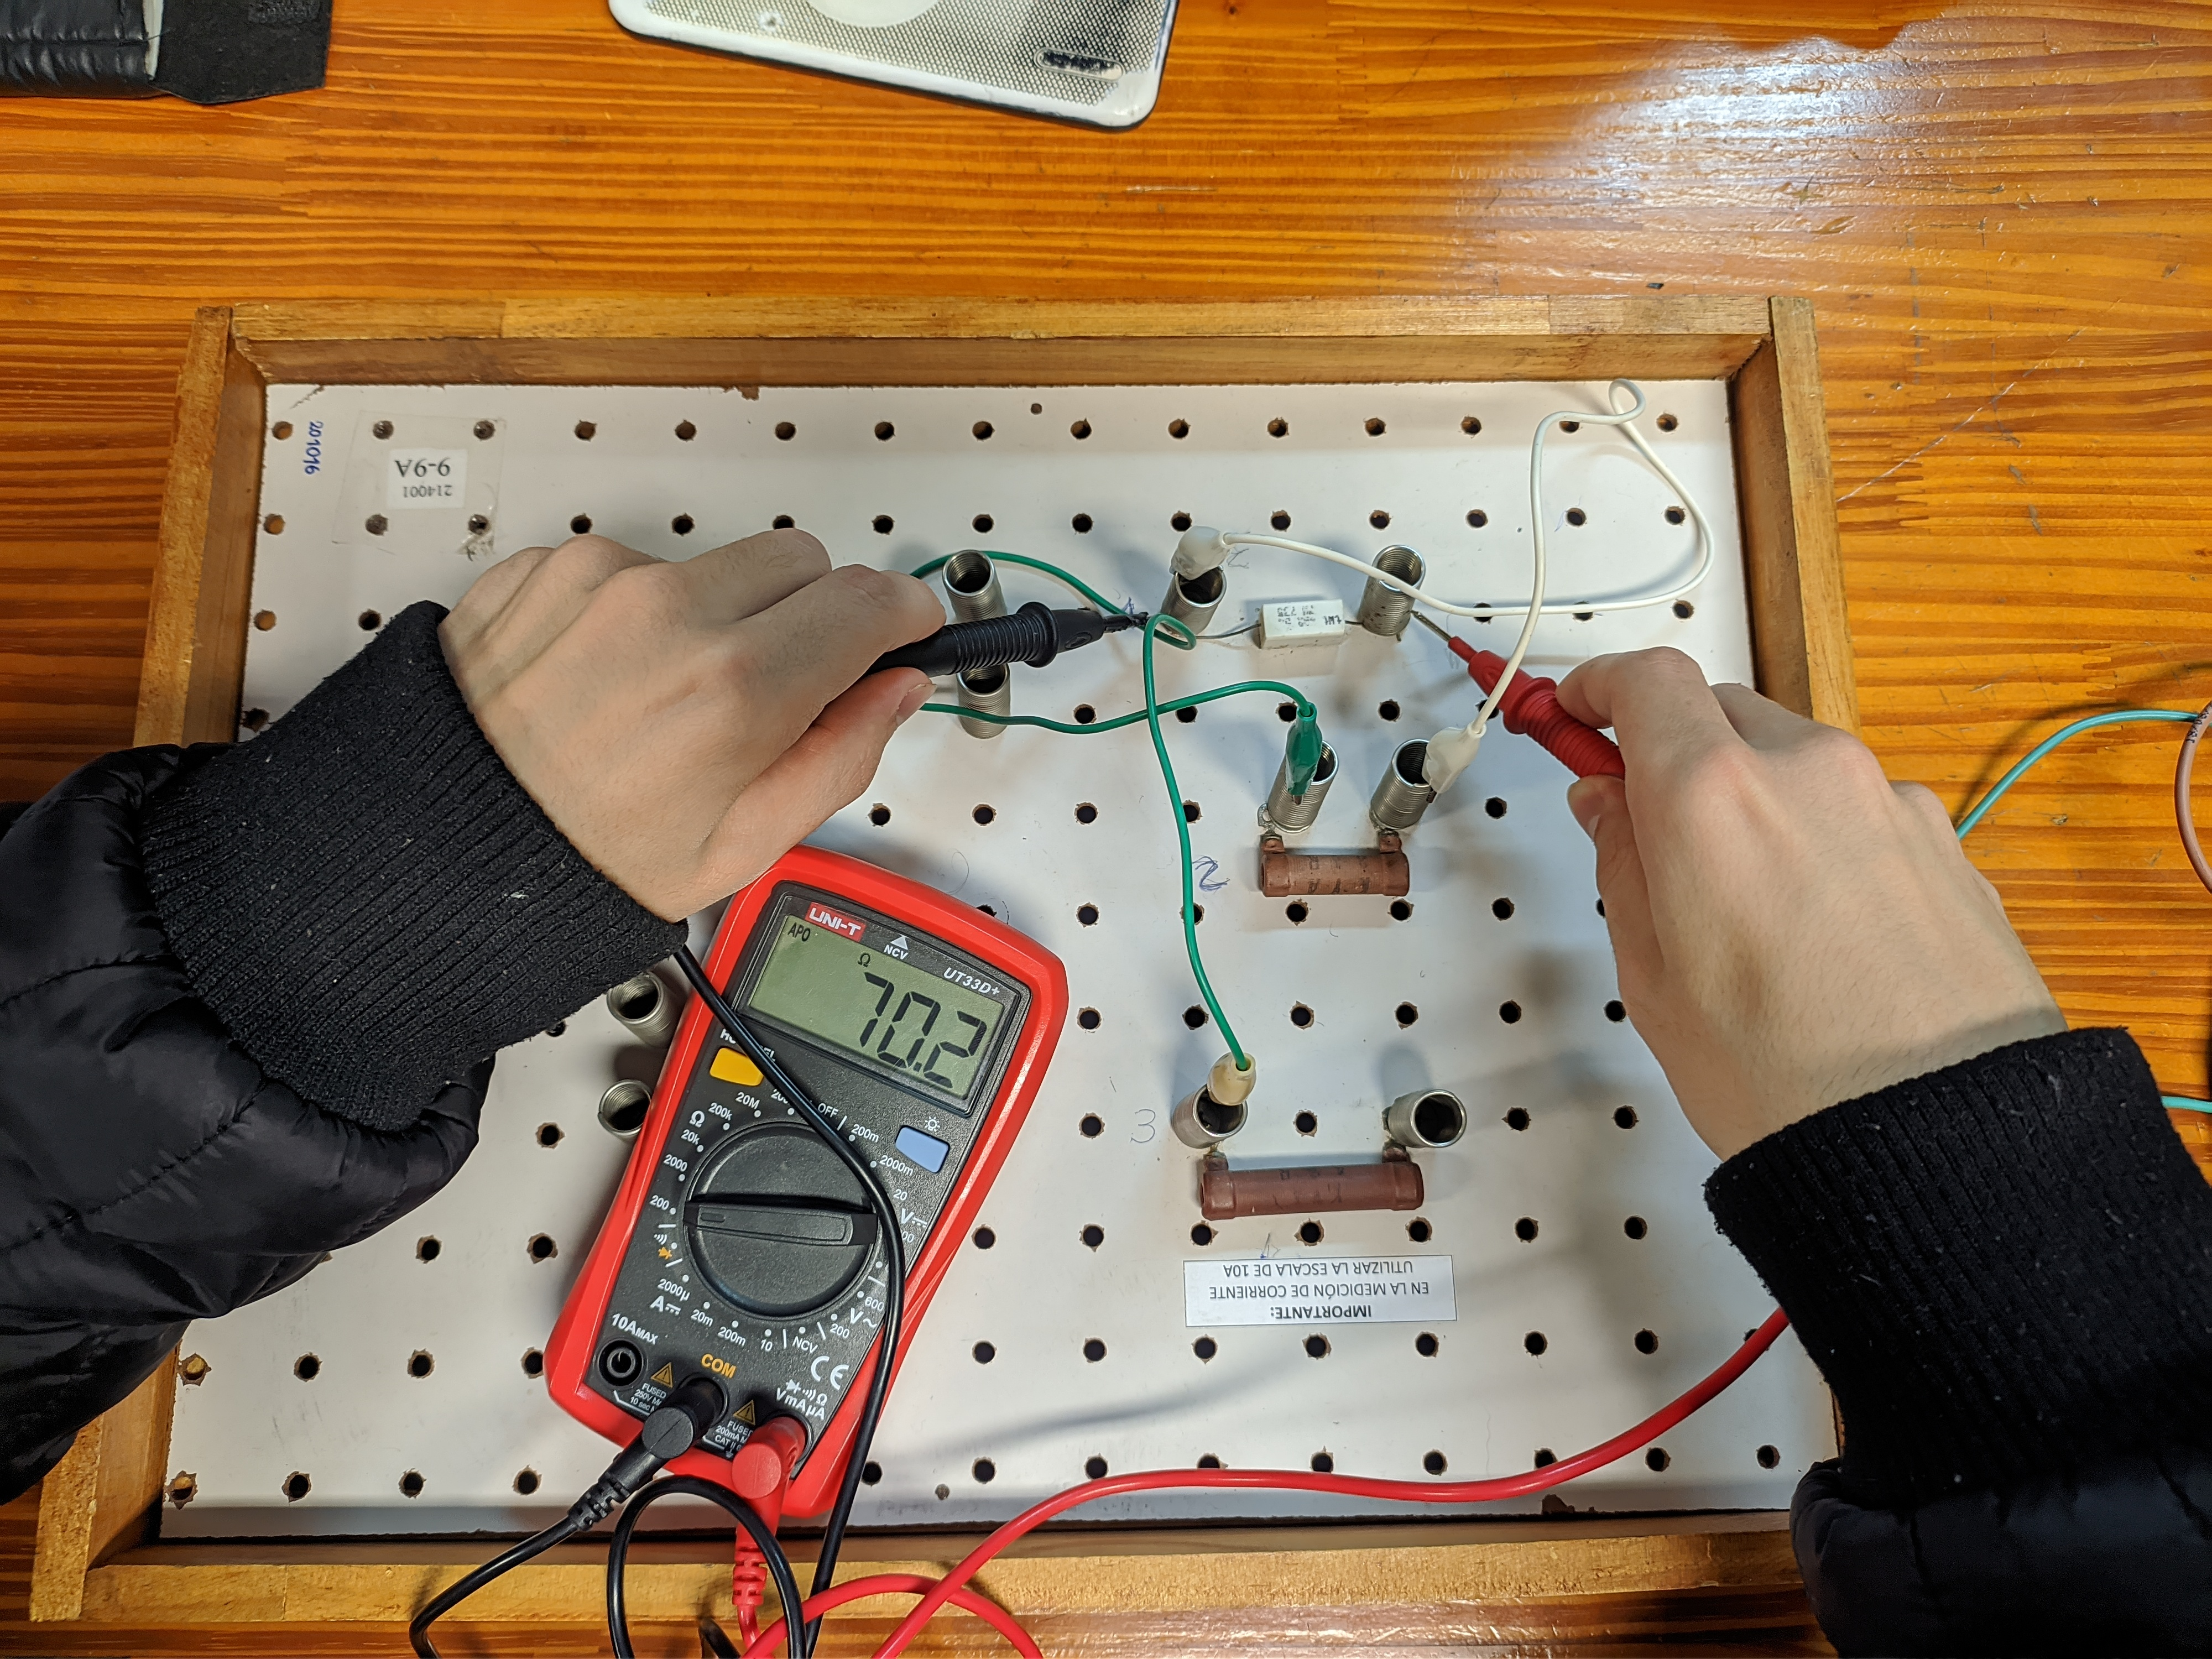
\includegraphics[width=1\textwidth]{./pictures/SERIE_R3.jpg}
    \textit{Medicion $R_3$.}
  \end{minipage}
\end{figure}

Con la medicion de la resistencia equivalente, observamos que se cumple la ecuación:

\noindent
\begin{figure}[h]
  \centering
  \begin{minipage}[h]{0.4\textwidth}
    \centering
    \vspace{-2em}
    $$R_{eq}=R_1+R_2+R_3$$
    $$R_{eq} = 151,\!6\Omega$$
  \end{minipage}\hskip 5mm
  \begin{minipage}[h]{0.4\textwidth}
    \centering
    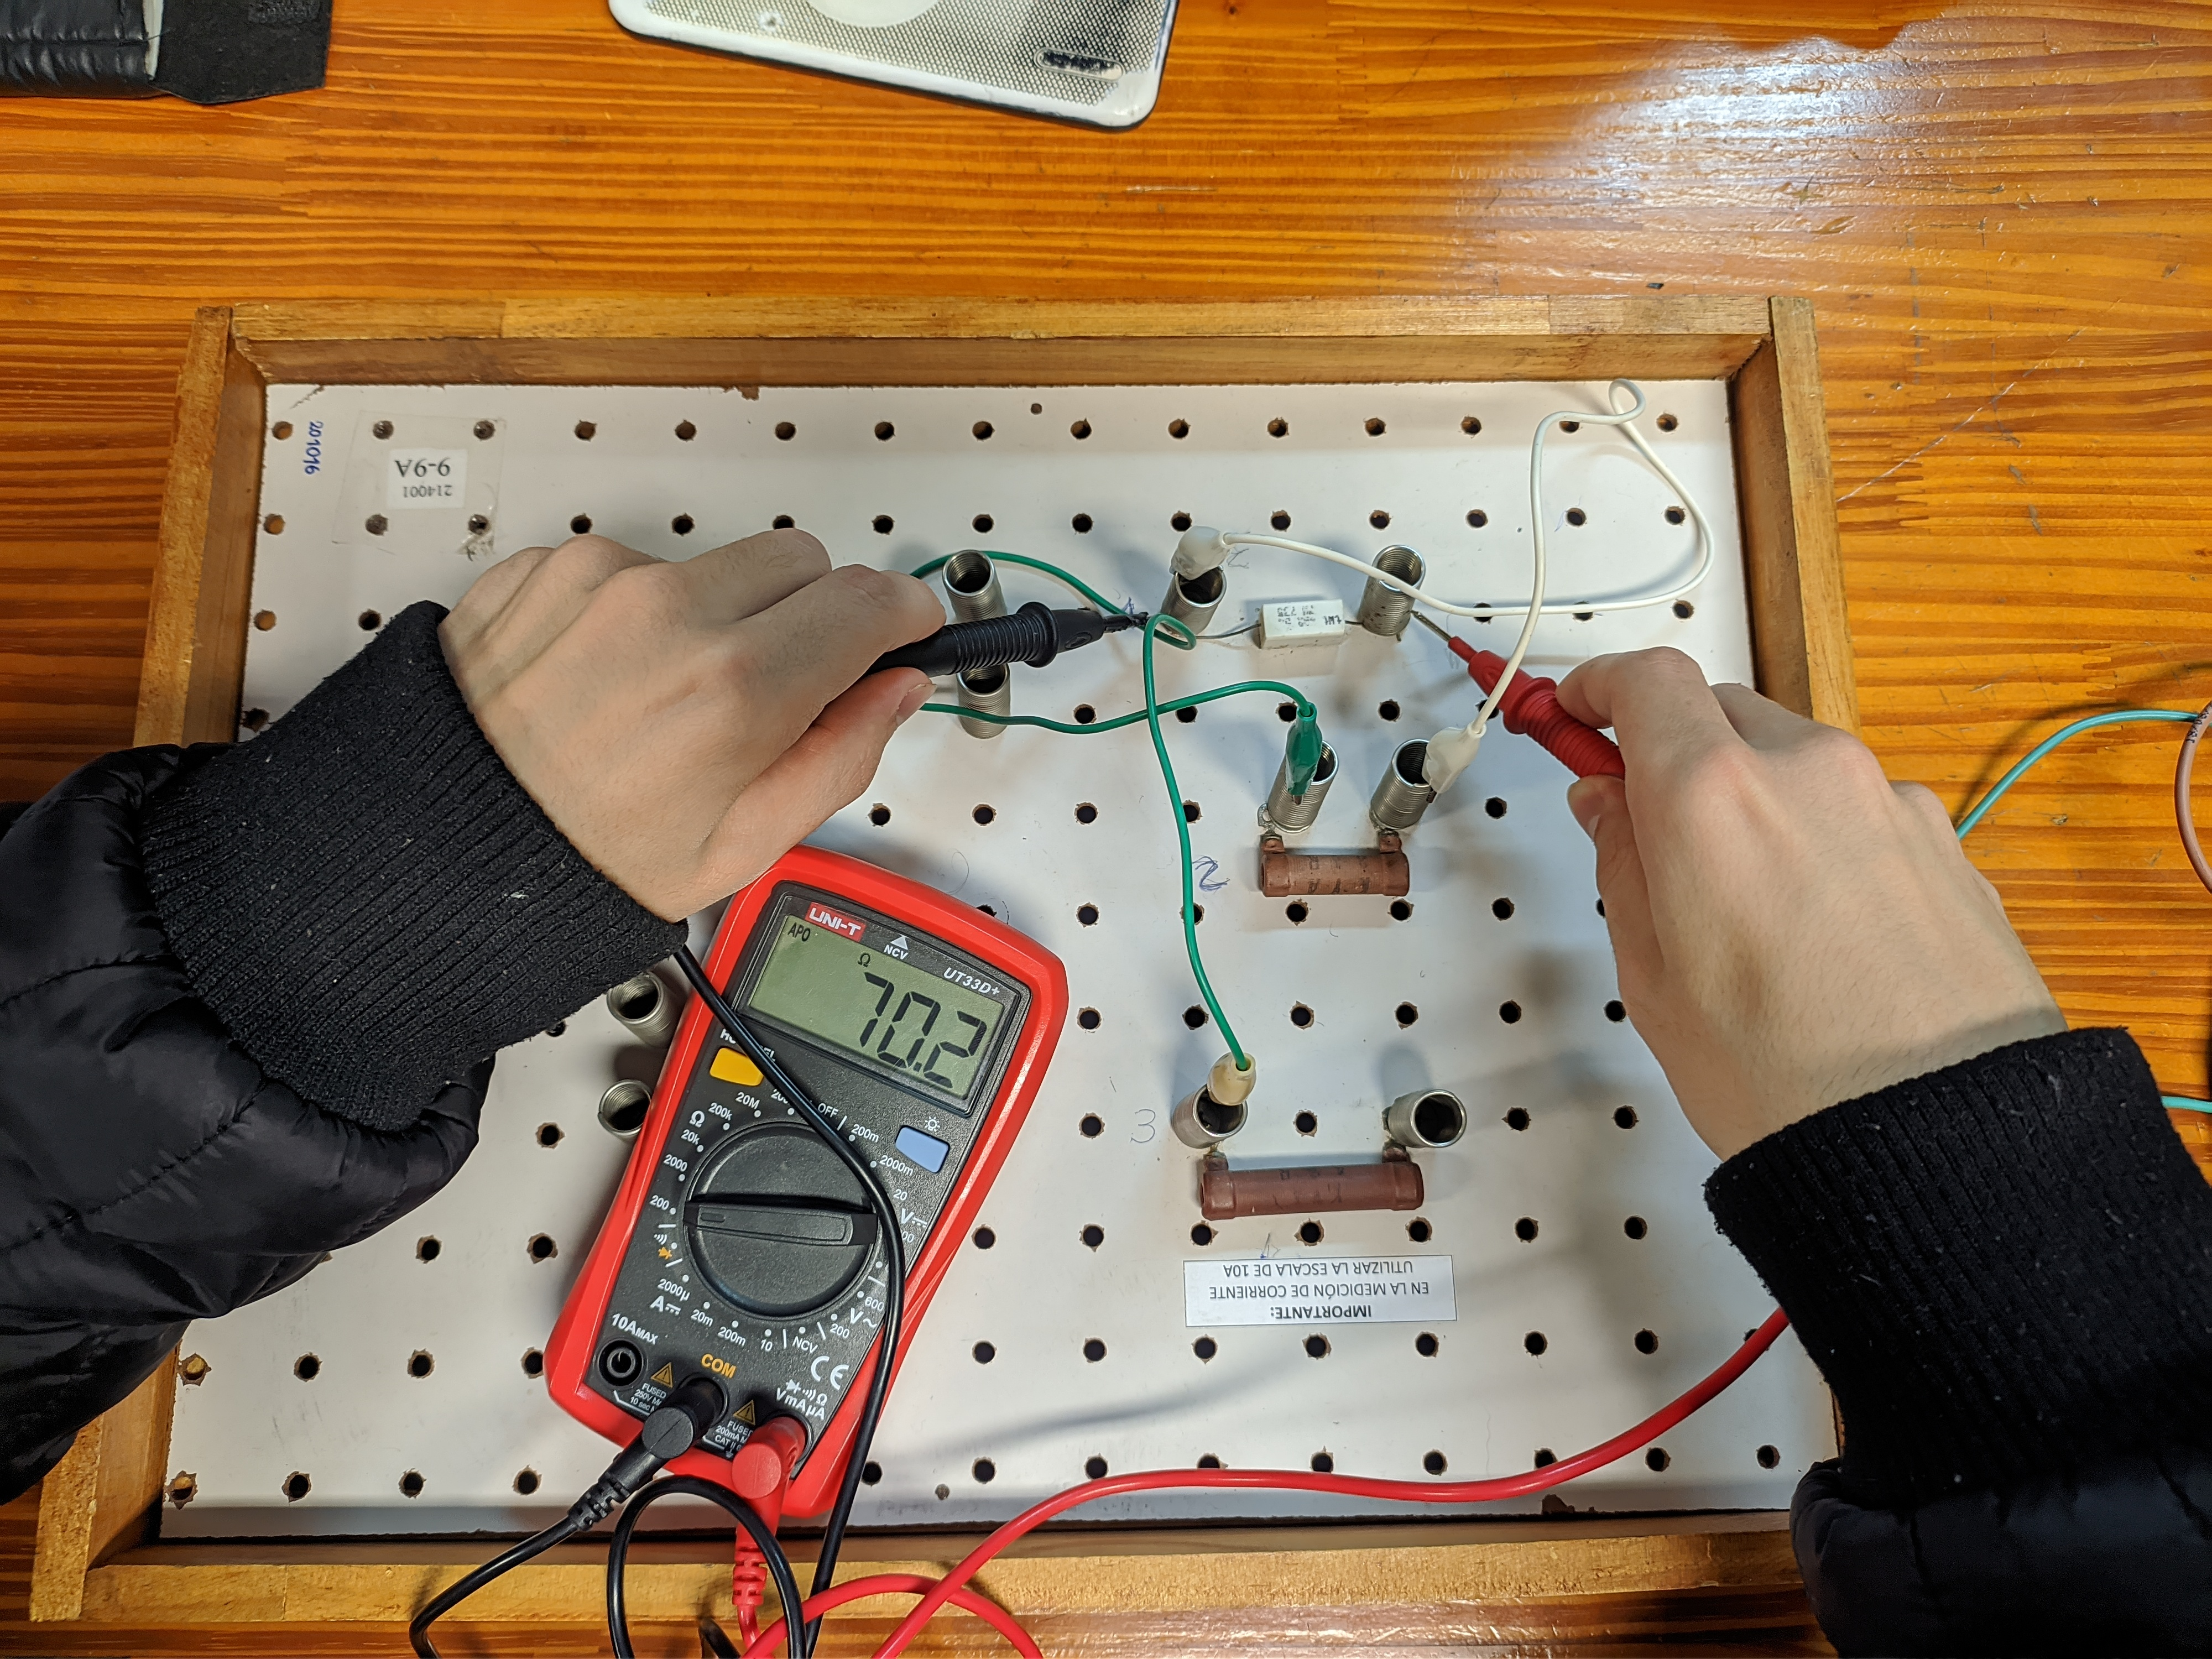
\includegraphics[width=1\textwidth]{./pictures/SERIE_R3.jpg}
    \textit{Medicion $R_{eq}$.}
  \end{minipage}
\end{figure}

Luego, se conectó la fuente al circuito, y se midio la tension entre sus bornes, obteniendo el
valor de:
\noindent
\begin{figure}[h]
  \centering
  \begin{minipage}[h]{0.4\textwidth}
    \centering
    \vspace{-2em}
    $$\LEpsilon = 15,\!43V$$
  \end{minipage}\hskip 5mm
  \begin{minipage}[h]{0.4\textwidth}
    \centering
    \includegraphics[width=1\textwidth]{./pictures/SERIE_fem.jpg}
    \textit{Medicion $\LEpsilon$.}
  \end{minipage}
\end{figure}

\section{Cálculos}

Una vez obtenidos estos datos, planteamos la ecuacion de Kirchoff del circuito,
con el objetivo de calcular la corriente y las caidas de tensión en cada resistor.

\begin{minipage}[t]{0.48\textwidth}
  $$
  \begin{aligned}
    0 &= \LEpsilon - V_{R_1} - V_{R_2} - V_{R_3}\\[6pt]
    0 &= \LEpsilon - I (R_1 + R_2 + R_3)\\[6pt]
    I &= \frac{\LEpsilon}{(R_1 + R_2 + R_3)}\\[6pt]
    I &= 101,\!78A\\[6pt]
  \end{aligned}
  $$
\end{minipage}
\hfill
\begin{minipage}[t]{0.48\textwidth}
  \vspace{7mm}
  $$
  \begin{aligned}
    V_{R_1} &= R_1 \cdot I = 4,\!9 V\\[6pt]
    V_{R_2} &= R_2 \cdot I = 3,\!47 V\\[6pt]
    V_{R_3} &= R_3 \cdot I = 7 V\\[6pt]
  \end{aligned}
  $$
\end{minipage}

Observamos que, como era esperado: $\LEpsilon =  V_{R_1} + V_{R_2} + V_{R_3}$. Esto 
indica que el valor de Corriente $(I)$ calculado es correcto. A pesar de eso, los valores de caida de tension que medimos difieren de los calculados debido a que los cables y las conecciones de los resistores agregan resistencia al circuito, disminuyendo la caida de tension por resistencia.

\noindent
\begin{figure}[h]
  \centering
  \begin{minipage}[h]{0.3\textwidth}
    \centering
    \includegraphics[width=1\textwidth]{./pictures/SERIE_VR1.jpg}
    \textit{Medicion $V_{R_1}$.}
  \end{minipage}\hskip 5mm
  \begin{minipage}[h]{0.3\textwidth}
    \centering
    \includegraphics[width=1\textwidth]{./pictures/SERIE_VR2.jpg}
    \textit{Medicion $V_{R_2}$.}
  \end{minipage}\hskip 5mm
  \begin{minipage}[h]{0.3\textwidth}
    \centering
    \includegraphics[width=1\textwidth]{./pictures/SERIE_VR3.jpg}
    \textit{Medicion $V_{R_3}$.}
  \end{minipage}
\end{figure}

Nota: Los valores presentados pueden no coincidir con los de las fotos porque fueron tomadas despues de la experiencia.

\chapter{Ejercicio 2}
Para la segunda experiencia, se armó el circuito a continuación.
\noindent
\begin{figure}[h]
  \centering
  \begin{minipage}{0.65\textwidth}
      \centering
      \begin{circuitikz}
          % Dibujar la fuente de voltaje
        \draw (0,0) to[battery1, l=$\LEpsilon$, invert] (0,4) -- (2,4)
        to[R, l=$R_1$] (2,0) -- (0,0);
        \draw (2,4) -- (4,4)
          to[R, l=$R_2$] (4,0) -- (0,0);
        \draw (4,4) -- (6,4)
          to[R, l=$R_2$] (6,0) -- (0,0);
      \end{circuitikz}
  \end{minipage}\hfill
  \begin{minipage}{0.35\textwidth}
      \centering
      (Valores teóricos)
      $$\LEpsilon = 16V$$
      $$R_1 = 50\Omega$$
      $$R_2 = 35\Omega$$
      $$R_3 = 70\Omega$$
  \end{minipage}
\end{figure}

\section{Procedimiento}

\subsection{Resistencia equivalente}

Calculamos y medimos las resistencia equivalente del circuito con la fuente desconectada.
Sabemos, de las mediciones del circuito anterior, que los valores reales de las resistencias son:

$$R_1 = 48,\!5\Omega \hspace{5mm} R_2 = 34,\!1\Omega \hspace{5mm} R_3 = 69\Omega \hspace{5mm}$$

Entonces:

\noindent
\begin{figure}[h]
  \centering
  \begin{minipage}[h]{0.4\textwidth}
    \centering
    \vspace{-2em}
    $$R_{eq}  = \left( \frac{1}{R_1}+\frac{1}{R_2}+\frac{1}{R_3} \right) ^{-1} = 15,\!51 \Omega$$\\
    La resistencia equivalente medida en el circuito fue de $R_{eq\hspace{1mm}real} = 17 \Omega$
  \end{minipage}\hskip 1cm
  \begin{minipage}[h]{0.4\textwidth}
    \centering
    \includegraphics[width=1\textwidth]{./pictures/PARALELO_Req.jpg}
    \textit{Medicion $R_{eq}$.}
  \end{minipage}
\end{figure}


\subsection{Corrientes}
Conectamos la fuente de alimentación y medimos la tensión que esta entregaba. Obtuvimos un valor de 
$ \LEpsilon=13,\!81 V $

Con este valor y el de las resistencias, podemos plantear las ecuaciones de Kirchoff de mallas y
nodos:

\[
\begin{cases}
  N_1 : I_{\LEpsilon} = I_{R_1} + I_{R_1} + I_{R_1} \\
  M_1 : 0 = \LEpsilon - I_{R_1} \cdot R_1 \\
  M_2 : 0 = I_{R_1} \cdot R_1 - I_{R_2} \cdot R_2 \\
  M_3 : 0 = I_{R_2} \cdot R_2 - I_{R_3} \cdot R_3
\end{cases}
\]

Resolviendo este sistema obtendremos el valor de las corritente a travez de cada resistencia

\noindent
\begin{minipage}[t]{0.33\textwidth}
  \centering
  De $M_1$ despejamos:
  $$I_{R1} = \frac{\LEpsilon}{R_1}$$
  $$I_{R1} = 284,\!74 mA $$
\end{minipage}
\begin{minipage}[t]{0.33\textwidth}
  \centering
  De $M_2$ despejamos:
  $$I_{R2} = \frac{I_{R_1}R_1}{R_2} $$
  $$I_{R2} = 404,\!98 mA $$
\end{minipage}
\begin{minipage}[t]{0.33\textwidth}
  \centering
  De $M_3$ despejamos:
  $$I_{R2} = \frac{I_{R_2}R_2}{R_3} $$
  $$I_{R3} = 200,\!14 mA $$
\end{minipage}

\vspace{7mm}

finalmente, a travez de la ecuacion N1, podemos obtener el valor de la corriente entregada 
por la fuente $\LEpsilon$
$$I_{\LEpsilon} = 889,\!86 mA$$

Obtenidas las corrientes a travez de cada una de las resistencias, podemos calcular su respectiva
caida de tensión:
$$ V_{R_1} = I_{R_1} \cdot R_1 = 13,\!8V \hspace{10mm} V_{R_2} = I_{R_2} \cdot R_2 = 13,\!8V 
\hspace{10mm} V_{R_3} = I_{R_3} \cdot R_3 = 13,\!8V $$

Observamos que la caída de tension es igual en todas las resitencias, lo cual era lo esperado, ya
que estan conectadas en paralelo. De esta forma, pudimos verificar nuestros resultados.

Por último, medimos la corriente entregada por la fuente $\LEpsilon$, observamos que el
valor mensurado es similar al valor calculado de forma teorica.

$$ I_{\LEpsilon \hspace{0,5mm} real} = 820mA \approx 889,\!86 mA $$

\noindent
\begin{figure}[h]
  \centering
  \begin{minipage}[h]{0.4\textwidth}
    \centering
    \includegraphics[width=1\textwidth]{./pictures/PARALELO_corr.jpg}
    \textit{Medicion $I$.}
  \end{minipage}\hskip 1cm
  \begin{minipage}[h]{0.4\textwidth}
    \centering
    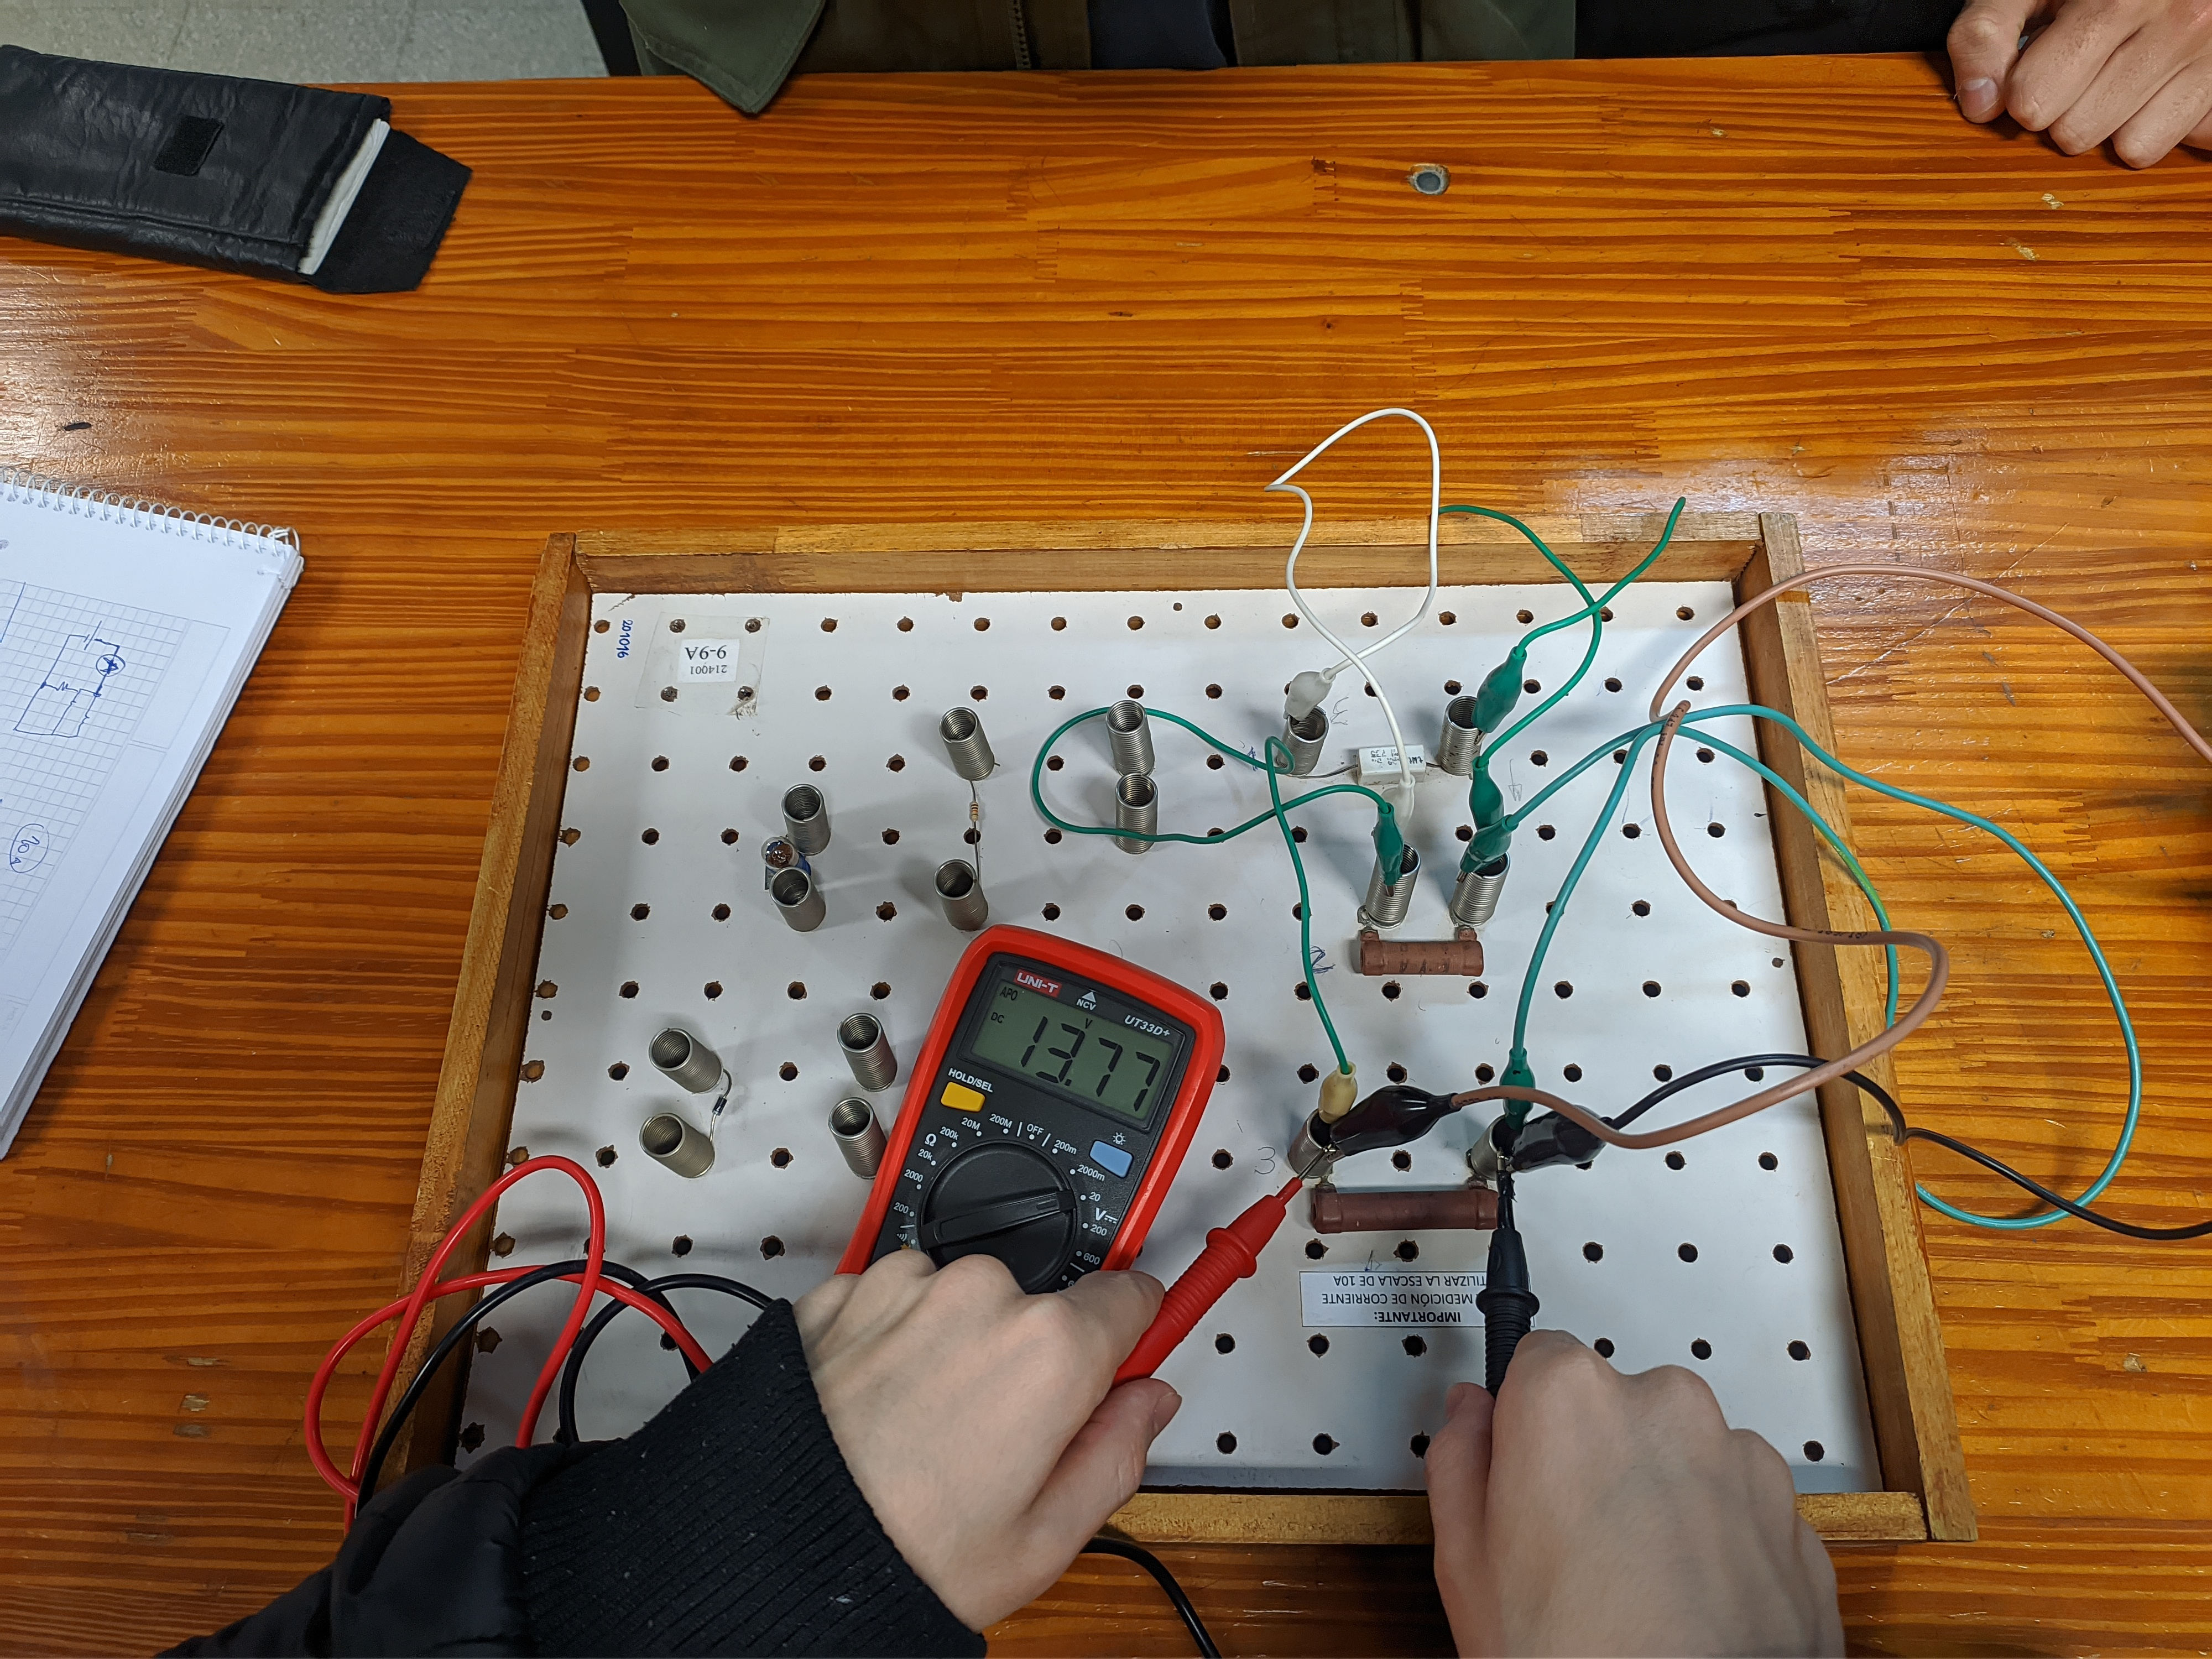
\includegraphics[width=1\textwidth]{./pictures/PARALELO_fem.jpg}
    \textit{Medicion $\LEpsilon$.}
  \end{minipage}
\end{figure}

Nota: Los valores presentados pueden no coincidir con los de las fotos porque fueron tomadas despues de la experiencia.

\chapter{Ejercicio 3}
\vspace{-0.5cm}
\noindent
\begin{circuitikz}
    \draw (0,0) to[voltmeter, l=$V_1$, ](0,3) -- (4,3)
    to[R, l=$R_2$](6,3) -- (9,3)
    to(9,3) -- (9,4);
    \draw (3,3) -- (3,5)
    to(3,5) -- (4,5)
    to[R, l=$R_3$] (6,5) -- (7,5)
    to[ammeter, l =$A_1$] (8,5) -- (9,5)
    to (9,5) -- (9,4);
    \draw (9,4) to[R, l=$R_4$](11,4) -- (12,4)
    to [battery1 ,l =$\LEpsilon_2$, invert] (14,4) -- (14,1)
    to [R ,l =$R_5$](14,-1) -- (14,-3)
    to [ammeter, l_=$A_2$, mirror](13,-3) -- (12,-3)
    to [R , l_=$R_6$](10,-3) -- (9, -3)
    to [battery1, l_=$\LEpsilon_3$](7, -3) -- (6, -3)
    to [R , l_=$R_7$](4,-3) -- (0, -3)
    to (0,0);
    \draw (3,-3) -- (3,-2)
    to [R ,l =$R_1$](3,-1) -- (3,1)
    to [battery1, l =$\LEpsilon_1$, invert] (3,2) -- (3,3);

    \node [above] at (8,0) {$\circlearrowright M_1$};
    \node [above] at (6,3.75) {$\circlearrowright M_2$};
\end{circuitikz}

$$
\begin{aligned}
    &R_1=3\Omega \hspace{2cm} && R_2=6\Omega \hspace{2cm} && R_3=3\Omega \hspace{2cm} && R_4=5\Omega\\[6pt]
    &R_5=2\Omega  &&R_6=1\Omega && R7=2\Omega\\[6pt]
    &\LEpsilon_1=50V &&\LEpsilon_2=28V  &&A_1=2A \\[6pt]
    &\LEpsilon_2=\,? &&V_1=\,? &&A_2=\,?\\[12pt]
\end{aligned}
$$
\vspace{-0.2cm}
$$
\left\{
\begin{array}{l}
\text{$I_1= I_2+I_3$} \\[6pt]
\text{$M_1: 0=50v-6\Omega \cdot I_3 - 5\Omega \cdot I_1+\LEpsilon -2\Omega \cdot I_1-1\Omega \cdot I_1-28-2\Omega \cdot I_1 -3\Omega \cdot I_1$} \\[6pt]
\text{$M_2: 0=-3\Omega \cdot I_2 +6\Omega \cdot I_3$}\\[6pt]
\end{array}
\right.
$$
\vspace{-0.5cm}
\begin{figure}[h]
 \begin{minipage}{0.4\textwidth}
  \centering
    $$
    \begin{aligned}
      M_1:\,&0=22V + \LEpsilon_2 -6\Omega \cdot 1A - 13\Omega \cdot 3A\\[6pt]
      &0=22V -45V + \LEpsilon_2\\[6pt]
      &\LEpsilon_2 = 23V\\[6pt]
      &\phantom{culo}
    \end{aligned}
    $$
  \end{minipage}\hfill
  \begin{minipage}{0.4\textwidth}
    \centering
    $$
    \begin{aligned}
      M_2:\,&0=3\Omega \cdot 2A + 6\Omega \cdot I_3\\[6pt]
      &I_3=\frac{6V}{6\Omega}=1A \\[6pt]
      &I_1=1A+2A=3A\\[8pt]
      & \text{Lectura del Amperimetro } A_2
    \end{aligned}
    $$
  \end{minipage}\hfill
\end{figure}


$$
\begin{aligned}
  &\LEpsilon_2=50v-3\Omega \cdot I_1\\[6pt]
  &\LEpsilon_2=50v -3\Omega \cdot 3A\\[6pt]
  &\LEpsilon_2=50-9v=41V\\
  &\text{Lectura del multimetro $V_1$}
\end{aligned}
$$

\chapter{Ejercicio 4}
\vspace{-1cm}
\noindent
\begin{circuitikz}
    \draw (0,-1) to[battery1, l =$\LEpsilon_1$, invert](0,3) -- (1,3)
    to[R , l=$R_1$](2,3)
    to[ammeter , l=$A_1$](6,3) -- (8,3);
    \draw (8,3) -- (8,2)
    to [R, l=$R_3$] (11,2)
    to [ammeter , l=$A_2$] (13,2)
    to (13,2) -- (13,4)
    to [R , l_=$R_2$] (8,4) -- (8,4)
    to (8,4) -- (8,3);
    \draw (13,3) -- (14,3)
    to [battery1, l =$\LEpsilon_2$] (14,-1) -- (14,-1)
    to (14,-1) -- (13,-1);
    \draw (13,-1) -- (13, -2)
    to[R , l_=$R_5$] (9,-2) -- (9,-2)
    to (9,-2) -- (9,0)
    to[R, l=$R_4$](13,0) -- (13, 0)
    to (13,-1);
    \draw (9,-1) -- (6,-1)
    to [battery1 , l_=$\LEpsilon_3$](3,-1)
    to [R, l_=$R_6$](1,-1)
    to (0,-1) -- (0,1);
    \draw (6,-1)to[voltmeter, l=$V_1$](6,3) -- (6,3);
    \draw (0,-1) -- (1,-2.5)
    to[voltmeter, l=$V_2$](5,-2.5) -- (6,-1);
    
    \node [above] at (3,0.75) {$\circlearrowright M_1$};
    \node [above] at (10.75,2.65) {$\circlearrowright M_2$};
\end{circuitikz}

$$
\begin{aligned}
    &R_1=5\Omega \hspace{2cm} && R_2=3\Omega \hspace{2cm} && R_3=6\Omega \hspace{2cm} && R_4=4\Omega\\[4pt]
    &R_5=12\Omega && R_6=2\Omega && R_7=2\Omega\\[4pt]
    &\LEpsilon_1=50V && \LEpsilon_2=30V && \LEpsilon_3=20V\\[4pt]
    &V_1=\,? && V_2=\,? && A_1=\,? && A_2=\,?\\[6pt]
\end{aligned}
$$

\[
\begin{cases}
  N_1 : I_1 = I_2 + I_3\\
  M_1 : 0 = E_1 - R_1 \cdot I_1 - R_{2//3} \cdot I_1 - \LEpsilon_2 - R_{4//5} \cdot I_1 + \LEpsilon_3 - R_6 \cdot I_1 \\
  M_2 : 0 = R_3 \cdot I_3 - R_2 \cdot I_2 \\
\end{cases}
\]\\

\noindent
\begin{minipage}[t]{0.5\textwidth}
  \centering
  De $M_1$ despejamos:
  $$0 = \LEpsilon_1 - \LEpsilon_2 + \LEpsilon_3 - (R_1 + R_{2//3} + R_6) \cdot I_1$$
  $$(R_1 + R_{2//3} + R_6) \cdot I_1 = \LEpsilon_1 - \LEpsilon_2 + \LEpsilon_3$$
  $$I_1 = \frac{\LEpsilon_1 - \LEpsilon_2 + \LEpsilon_3}{(R_1 + R_{2//3} + R_6) \cdot I_1}$$
  $$I_1 = \frac{40 V}{12 \Omega} = 3,\!34 A$$
  Lo anterior es lo medido por el $A_1$
\end{minipage}
\begin{minipage}[t]{0.5\textwidth}
  \centering
  Sabiendo que:
  $$I_2 = I_1 - I_3$$
  De $M_2$ despejamos:
  $$0 = R_3 \cdot I_3 - R_2 \cdot (I_1 - I_3)$$
  $$0 = (R_3 + R_2) \cdot I_3 - R_2 \cdot I_1$$
  $$(R_3 + R_2) \cdot I_3 = R_2 \cdot I_1$$
  $$I_3 = \frac{R_2 \cdot I_1}{R_3 + R_2}$$
  $$I_3 = \frac{10,\!02 V}{9 \Omega} = 1,\!113 A$$
  Lo anterior es lo medido por el $A_2$
\end{minipage}

\newpage

Para el calculo de los voltajes, procedemos por aislar los elementos entre las "puntas" de los voltimetros, y sus caidas y aportes de tension son lo que el voltimetro va a leer:\\

\noindent
\begin{minipage}[t]{0.5\textwidth}
  \centering
  Para el $V_1$:
  $$\Delta V = \LEpsilon_3+R_6 \cdot I_1 + \LEpsilon_1 - R_1 \cdot I_1$$
  $$\Delta V = 46,\!69 V = V_1$$
\end{minipage}
\begin{minipage}[t]{0.5\textwidth}
  \centering
  Para el $V_2$:
  $$\Delta V = \LEpsilon_3 - R_6 \cdot I_1$$
  $$\Delta V = 13,\!34 V = V_2$$
\end{minipage}

\end{document}


